%%==================================================
%% chapter01.tex for BIT Master Thesis
%% modified by yang yating
%% version: 0.1
%% last update: Dec 25th, 2016
%%==================================================
\chapter{绪论}
\label{chap:intro}
\section{本文研究的目的和意义}
在未来战争中,仅靠单架无人机自主作战无法适应复杂多样的战场环境,而具备协同作战的无人机编队能更好地完成任务,与单架无人机相比具有作战效率高、
视野广阔等优势,可实现对目标的全方位立体监视,对地精确攻击。另外,无人机紧密编队可以实现长航任务中无人机的空中加油,对接等任务,如图\ref{fig:c01-meaning}。
编队飞行作为无人机研究领域的热点与难点问题,涉及多项关键技术,例如:队形设计、自主编队、队形保持变换、协调通信等。无人机自主编队控制是实现集群作战的关键技
术。

固定翼无人机以紧密编队的形式飞行,如迁徙的鸟儿一样,可以减少整体的飞行阻力并且减少燃料消耗。整体编队产生的效果将会与精心设计的、具有良好的气动
外形的飞行器相媲美。但是,按照相关文献显示,如果固定翼编队的控制精度无法达到要求精度的10\%,那么最优的减租效果可能会被削减30\%。
 \begin{figure}[H]
  \centering
  \subfigure[无人机编队加受油]{
  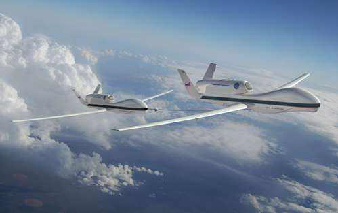
\includegraphics[width=0.45\textwidth]{figures/c1/c01-meaning-1.png} 
}
  \subfigure[无人机编队巡航]{
  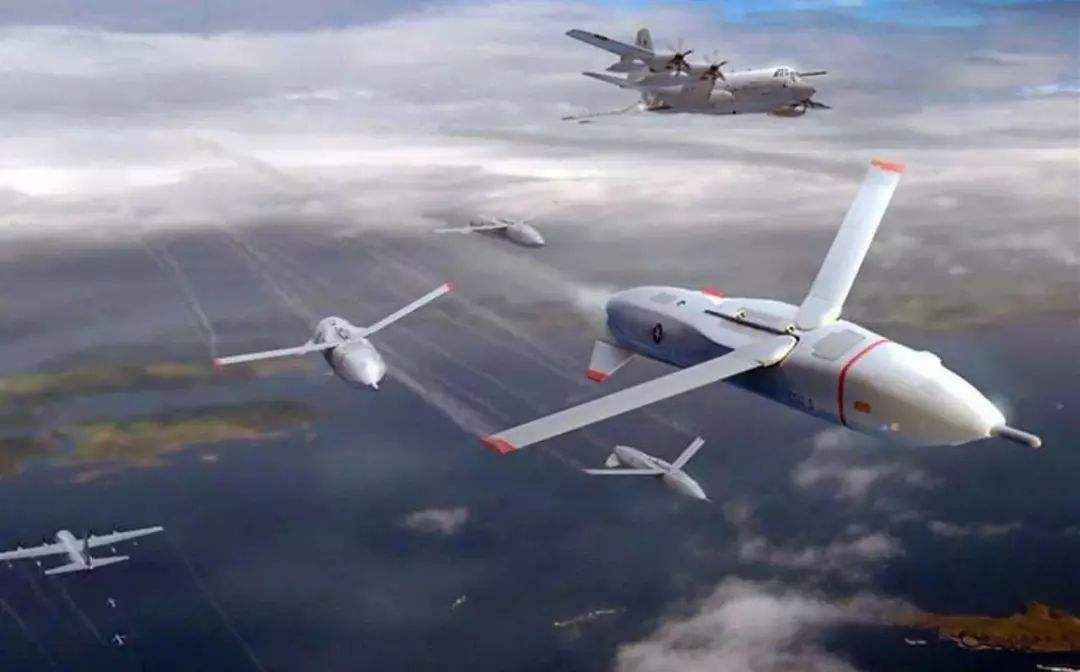
\includegraphics[width=0.45\textwidth]{figures/c1/c01-meaning-2.jpeg}
}
  \caption{无人机编队应用场景}
  \label{fig:c01-meaning}
  \end{figure}
%\upcite{Takahashi1996Structure,Xia2002Analysis,Jiang1989,Mao2000Motion,Feng1998}%这个是文献引用上标
\section{国内外研究现状及发展趋势}
%\label{sec:***} 可标注label
现如今的无人机自动驾驶仪的结构由导航模块、位置控制控制模块(外环)以及姿态控制模块(内环)组成;导航模块产生期望位置,位置控制模块由期望位置产生
期望姿态角,姿态控制模块由期望姿态角产生最终的伺服系统的控制量。现如今的低成本无人机所使用的传感器硬件精度比较低,均为消费级别,如果不考虑传感
器的精度问题而设计控制方案,很可能导致整体编队的控制精度下降。现如今已经存在的大部分编队控制算法均为考虑飞机的质点运动学以及质点动力学条件下提
出的导航方法,最终产生的飞行器的控制量为无人机航迹坐标系下的加速度期望值以及飞机的航向角的期望角速度。按照飞机的控制方式,需要将航迹坐标系下的
期望控制量转到机体系之下,但是飞机自动驾驶仪并不能接受加速度控制量,尤其是飞机机体$O_bx_b$轴方向,无人机推力、阻力以及重力沿机体方向的推力并非是代数关
系,不能直接由期望加速度得到期望推力;无人机姿态驾驶仪常使用协调转弯模型作为内环角度环的控制基础,不能直接响应所给出的偏航角速度的期望值。另外由于低成
本无人机的惯性原件的精度问题导致无人机不能使用测量的加速度信息作为反馈,两种原因导致以加速度
为最终控制量对于低成本无人机编队的方法控制精度不足。

%TODO:此处的引用存疑
目前的编队控制已经提出多种方案,例如:基于距离的编队控制策略、人工势场法,基于距离的编队控制,基于行为的编队控制,基于虚拟结构的编队控制,基于虚
拟领机的编队控制等。其中,基于距离编队中的领从模式因其原理简单而得到广泛应用。本文正是基于领从策略(leader-follower method)设计的编队控制器。
\section{本文的技术方案}
%\label{sec:***} 可标注label
首先建立无人机编队的领机与从机相对运动模型,描述领机从机在三维空间之内的运动规律。其次按照编队的控制目标设计编队控制器的误差输入量,并按照无人机
的内环的输入量,设计编队控制的数学形式。之后再完成无人机质点模型下的编队控制率仿真,完善编队所设计编队控制器的结构。之后,利用ROS/Gazebo等仿真包搭建
无人机编队动力学仿真环境,测试编队控制再考虑自动驾驶仪内环以及无人机的动力学模型之后的编队控制表现。最后,进行实际飞行的测试:记录编队控制的实际动态特性
稳态特性、飞行编队的抗干扰能力、以及编队的能源节约情况。
\section{本文的组织结构}
本文之后的部分将如下组织:第二章建立无人机编队的动力学模型;第三章设计编队控制器数学形式;第四章介绍无人机编队整体控制逻辑、仿真环境以及硬件选型
;第五章控制器仿真以及实际飞行实验结果分析;第六章为结论。